Many different disciplines use motion analysis systems to capture human body movement and posture. Basic scientists want to learn more about the mechanisms that are used to translate muscular contractions about articulating joints into functional accomplishments like walking. Researchers are increasingly attempting to better understand the relationship between the human motor control system and gait dynamics.

Motion capture \cite{Review on Motion Capture Technology} is now widely used in the gaming, film, and animation industries to provide quick, low-cost body and/or facial animations in order to animate one or more characters. Animation processes did not see significant innovation until computers were introduced into the process. With the invention of key-framing, which reduced the number of samples required to create an animation, animators' jobs became much easier. This was a time-consuming process because, at the time, each artist was required to individually animate each pose/frame. With the introduction of key-framing, the artist specified the beginning and ending frames of the animation, while the intermediate frames of the movement were generated automatically. Some animations, however, remained impossible to recreate due to their inherent complexity, such as the human walking animation, which is too complex due to our articulations.

\begin{figure}[h]
	\centering
	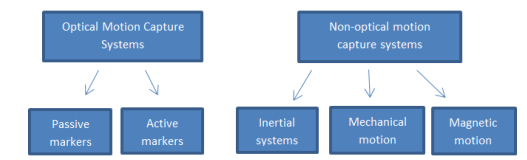
\includegraphics[width=0.7\textwidth]{figures/Mocap.png}
	\caption{MoCap systems Hierarchy}
\end{figure}

Motion analysis data collection protocols, measurement precision, and data reduction models have all been developed to meet the needs of their respective settings. Sport assessments, for example, necessitate higher data acquisition rates due to higher velocities than normal walking. Furthermore, real-time tracking is required for a realistic user experience, so time lag should be kept to a minimum. Years of technological advancement have resulted in numerous systems that can be classified as optical and non-optical, where non-optical category contains mechanical, magnetic, or inertial trackers. The human body is frequently viewed as a network of rigid links connected by joints. Human body parts are not rigid structures, but they are commonly treated as such during human motion studies.